%%%%%%%%%%%%%%%%%%%STETTINGS%%%%%%%%%%%%%%%%%%%%%%%%%%%%%%
\documentclass[12pt]{report}
\usepackage{hyperref}
\usepackage[style=verbose, autocite=footnote, backend=biber]{biblatex}
\addbibresource{ref.bib} 
\usepackage{graphicx} 
\usepackage[utf8]{inputenc}
\usepackage[T1]{fontenc}
%\usepackage[french]{babel}
\usepackage[greek,french]{babel}
\usepackage[margin=2.5cm, left=3.5cm]{geometry}
\usepackage{setspace}
\usepackage{titlesec}
\usepackage{comment}
\usepackage[export]{adjustbox}
\usepackage{pdfpages}


%%%%%%%%%%%%%%%%%%%%%%%%%%%%%%%%%%%%%%%%%%%%%%%%%%%%%%%%
	\titleformat{\section}{}{}{0em}{\bf\LARGE}
	\titleformat{\subsection}{}{}{0em}{\bf\Large}
	\titleformat{\subsubsection}{}{}{0em}{\bf\normalsize}
 
\titleformat{\chapter}[hang]{\bf\huge}{\thechapter}{2pc}{}


%%%%DOCUMENT%%%%

%%\setcounter{tocdepth}{6}
\begin{document}

    \begin{titlepage}
        \begin{center}
        
\includegraphics[width=0.1\textwidth, margin= 0 -1.5cm 0 0]{l.jpg}
        
\includegraphics[width=0.8\textwidth]{u.jpg}
        \vspace{0.5cm}
      \newline Faculté de Lettres, Traduction et Communication
     \end{center}
     \vspace*{1cm}
     Master Sciences et Technologies de l'Information et de la Communication
     \newline STIC-B415  Architecture des systèmes d'information 
       \vspace*{0,5cm}
        \newline Professeur : Sébastien de Valeriola
        \newline Assistant : Guillaume Quintin
     \newline A rendre pour le 8 janvier 2024.
      \vspace*{0,5cm}
     \newline \rule{11cm}{0,02cm}
     \vspace*{1,5cm}
     \newline \textbf{{\Large Le développement et l'application d'ontologies dans le contexte archivistique}}
       \vspace*{0,5cm}
        %\vspace*{0,5cm}
     \vspace*{1cm}
     \newline Chloé Steylaers
     \newline 000427498
     \vspace*{1,5cm}
     \newline \rule{4cm}{0,02cm}
\end{titlepage}
\newpage
\tableofcontents
\newpage
\chapter{Introduction}
Dans un monde où les technologies de l'information évoluent à une vitesse fulgurante, l'archivistique se trouve à un carrefour crucial. Historiquement enracinée dans des pratiques anciennes, cette discipline doit désormais s'adapter aux changements radicaux apportés par l'ère numérique. Notre étude se propose d'explorer le développement et l'application d'ontologies dans ce contexte archivistique, mettant en lumière la transformation dynamique de cette discipline.

Nous débuterons par une analyse du concept du web sémantique, un élément clé dans l'évolution du web. Son rôle dans l'extension des capacités du web actuel sera examiné, notamment sa contribution à l'amélioration de l'accès et de l'interopérabilité des données.

Nous poursuivrons ensuite l'étude avec un examen des ontologies, abordant à la fois leurs fondements philosophiques et leurs applications pratiques en informatique et intelligence artificielle. Cette partie de l'étude vise à comprendre comment les principes philosophiques ont influencé les développements technologiques, en particulier dans le domaine de l'intelligence artificielle symbolique.

Ensuite, nous examinerons la transition des modèles classificatoires traditionnels aux modèles conceptuels dans le domaine du patrimoine culturel. Cette section met en évidence l'importance croissante des modèles conceptuels pour la gestion efficace de l'information et pour l'interopérabilité entre divers systèmes d'information culturelle.

Nous nous concentrerons ensuite sur le modèle \textit{Record in Contexts} (RiC), avec ses deux éléments principaux, RiC-CM (Conceptual Model) et RiC-O (Ontology). Nous discuterons de leur rôle dans la modernisation de l'archivistique et examinons les défis liés à leur mise en œuvre, notamment en termes d'alignement avec les systèmes existants, de financement, et de formation des professionnels.

Enfin, nous évoquerons les critiques et les préoccupations soulevées autour du RiC, notamment en ce qui concerne sa complexité et les inégalités potentielles dans son application.

\newpage
\chapter{Les évolutions de l'archivistique}
La conservation de traces liées à l'humanité représente une pratique extrêmement ancienne, antérieure même à l'invention de l'écriture. Cette activité, variante selon les cultures et les époques, a connu une évolution significative. L'archivistique, telle que nous la comprenons actuellement, surtout dans nos régions, trouve ses racines aux 17e et 18e siècles, avec une spécialisation accrue au cours du 19e siècle. En tant que discipline, l'archivistique évolue en parallèle avec les sociétés qui la façonnent, influençant ainsi la gestion de l'information archivistique, la nature même de l'archive, ainsi que les concepts fondamentaux régissant sa conservation et son archivisation (c'est-à-dire sa préservation et sa mise à disposition).

Au 19e siècle, des principes tels que le respect de l'intégrité et de la provenance des documents ont été établis, sur lesquels se sont greffées des pratiques descriptives des fonds d'archives. Parmi ces pratiques, la norme ISAD-(G) se distingue par sa description hiérarchique d'un document ou d'un fonds d'archives. Aujourd'hui, la communication entre les différentes disciplines travaillant avec les archives, principalement les archivistes et les historiens, est devenue plus complexe en raison de la spécialisation croissante de ces domaines.

Cette complexification disciplinaire s'accompagne des défis contemporains liés à la gestion d'une quantité colossale d'archives. La conservation de formats matériels tels que le papier pose des enjeux d'espace et de gestion, tandis que l'augmentation des archives numériques soulève des questions de pérennité.

En outre, l'avènement du web et des ressources en ligne a profondément transformé les systèmes d'information, rendant accessibles de vastes quantités de ressources de manière inédite. Les domaines des archives, des bibliothèques et des autres sciences du patrimoine ne sont pas restés en marge de ces évolutions. En s'adaptant aux changements sociétaux, ces disciplines cherchent à améliorer les systèmes de transmission des connaissances et l'accessibilité de leurs collections.
\chapter{Le web sémantique}
Dans le cadre évolutif du World Wide Web et de ses outils, une réflexion approfondie a été menée autour des données liées (\textit{linked data}) et du développement d'ontologies spécifiques aux domaines du patrimoine culturel et historique. Le concept du web sémantique, bien qu'il ne soit pas entièrement récent dans le contexte des avancées technologiques, a été introduit par Tim Berners-Lee au tournant du 21e siècle. Fondamentalement, le web sémantique, également désigné sous le terme de web 3.0 ou encore web de données par opposition au web des documents, vise à étendre les capacités du web actuel en facilitant l'accès et l'interopérabilité des données. Cette avancée est marquée par l'adoption de technologies favorisant une structuration, une connexion et une interprétation améliorées des données web.

Au cœur du web sémantique se trouve la standardisation des données, rendue possible par des langages tels que le RDF (Resource Description Framework) et l'OWL (Web Ontology Language). Ces outils sont essentiels pour établir des relations complexes entre les données, facilitant ainsi la création de métadonnées qui sont interprétables tant par les humains que par les machines.

L'ontologie représente une méthode formelle pour définir les types, les propriétés et les relations entre les entités, permettant ainsi aux machines de traiter et d'interpréter le contenu du web de manière plus raffinée. Cette capacité améliore significativement la recherche et l'extraction de données, en fournissant des résultats plus pertinents et précis.
De plus, le web sémantique ambitionne de rendre les données plus connectées et intégrées. Par le biais de liens sémantiques, il est en effet possible d'agréger des informations issues de sources variées pour obtenir une perspective complète et détaillée sur un sujet donné.

Cependant, la mise en œuvre du web sémantique présente des défis, notamment en termes de conception d'ontologies robustes et de la gestion de la confidentialité et de la sécurité des données. Malgré ces difficultés, le potentiel du web sémantique pour révolutionner la façon dont nous accédons et utilisons les informations en ligne est immense, ouvrant la voie à des applications plus intelligentes et intuitives.

\chapter{Les ontologies}
Afin d'appréhender pleinement le concept d'ontologie formelle, il peut être intéressant de se plonger dans les fondements philosophiques de ce terme. L'ontologie, dans le contexte de la philosophie occidentale, est un champ d'étude spécifique qui s'intéresse à l'existence, à la nature et à la structure de la réalité. Bien que le terme "ontologie" ne soit apparu qu'au XVIIe siècle, les questionnements relatifs à l'existence, la réalité, et l'être, qui sont au cœur de cette discipline, remontent aux origines mêmes de la philosophie occidentale, presque aussi anciennes que les premiers écrits philosophiques reconnus traditionnellement.

\section{En philosophie}
L'ontologie (de onto-, tiré du grec \textgreek{ὤν, ὄντος} « étant », participe présent du verbe \textgreek{εἰμί} « être ») joue de ce fait un rôle primordial dans le web sémantique. Ce terme est emprunté à la philosophie et désigne dans ce contexte le discours et questionnement relatif à l'être, l'étant. 

Bien que l'étymologie de ce terme concerne étymologique l'étude de l'être, la définition exacte de ce que recouvre ce champ d'étude de l'ontologie est loin d'être sans équivoque. Cela implique une exploration profonde des catégories de l'existence, non seulement en interrogeant ce qui existe, mais aussi en sondant la nature de cette existence. Comment les choses existent-elles ? Quelles sont les caractéristiques fondamentales de l'être ? Il existe de fait différentes perspectives sur le rôle de l'ontologie. Pour certains, elle est chargée d'examiner l'existence, visant à dresser un inventaire de tout ce qui existe. D'autres la voient comme une étude des propriétés fondamentales de l'être, se concentrant sur les relations entre les entités existantes. D'autres approches encore, considèrent l'ontologie comme une analyse de l'engagement ontologique inhérent à diverses théories ou langages, qu'ils soient scientifiques, courants, ou autres\autocite{arapinis2018ontologie} .
Par ailleurs, souvent perçue comme un sujet "vieux comme le monde", elle constitue un pan majeur de la philosophie occidentale.

De Platon et Aristote, qui posaient les premières pierres de la métaphysique, à des penseurs contemporains qui continuent de repousser les frontières de cette discipline, l'ontologie est restée un domaine vital et constamment évolutif de la philosophie. Sa richesse et sa complexité reflètent la perpétuelle quête humaine de compréhension de la réalité dans son ensemble.

Aujourd'hui, l'ontologie maintient son importance en philosophie, tout en inspirant et en influençant d'autres domaines, notamment l'intelligence artificielle et la mise en place de structure de données dans le systèmes d'information.
 
\section{L'ontologie formelle}
Le concept d'ontologie formelle, crucial dans le domaine de l'intelligence artificielle, s'est façonné et développé parallèlement aux avancées scientifiques du XXe siècle. Ce concept entretient une relation étroite avec la logique formelle\footnote{Cette discipline, influencée par l'école de pensée logiciste, présente des définitions variées selon les philosophes et les courants de pensée. Elle peut être envisagée comme l'étude des langages artificiels et de leurs structures, l'analyse des inférences logiques et de leurs conséquences, ou encore comme l'examen des principes généraux du jugement.}, dont les développements prolifiques ont marqué le début du XXe siècle. Les travaux d'Edmund Husserl, notamment ses \textit{Recherches Logiques}, ont exercé une influence notable dans ce champ. La première moitié du XXe siècle a été caractérisée par des progrès significatifs en logique formelle, avec des contributions majeures de figures telles que George Boole, pionnier en algèbre logique, ainsi que Bertrand Russell et Alfred North Whitehead, dont l'œuvre monumentale \textit{Principia Mathematica} a constitué un jalon essentiel dans la compréhension formelle des structures mathématiques. De plus, les réflexions de Gottlob Frege et les travaux du Cercle de Vienne ont joué un rôle crucial dans l'évolution de ces idées.

L'ontologie formelle, tout comme la logique formelle en philosophie, cherche à établir les conditions de possibilité d'une théorie. Cette démarche s'inscrit dans l'héritage de la pensée de Leibniz concernant une \textit{Characteristica Universalis}, c'est-à-dire l'idée de formaliser dans un langage universel l'ensemble des concepts mathématiques, scientifiques et métaphysiques. Ce langage serait fondé sur un \textit{calculus ratiocinator}, permettant de résoudre les problèmes de raisonnement par des calculs, et visant ainsi à mettre fin aux débats ou oppositions de raisonnements.

En résumé, cette période de l'histoire de la philosophie a été marquée par un vif intérêt pour le logicisme et l'idée que la logique pourrait révéler la structure ontologique profonde des choses. Ce mouvement est étroitement lié au développement des mathématiques à la fin du XIXe siècle. La genèse de la logique formelle peut être perçue comme émanant du programme logiciste, et en particulier de la philosophie arithmétique de Frege, développée dans le but de fournir des fondements solides à l'arithmétique, en démontrant que les nombres qu'elle postule peuvent être dérivés de lois logiques.

\section{De la philosophie à l'informatique}
Dans la continuité des avancées technologiques et scientifiques du milieu du XXe siècle, l'intelligence artificielle (IA) a commencé à s'établir comme un domaine de recherche distinct, notamment à partir de la conférence de Dartmouth en 1956. Cette conférence est fréquemment citée comme le point de départ, voire la naissance officielle, de l'intelligence artificielle en tant que discipline académique à part entière.

Au sein de la recherche en IA, divers courants de pensée et paradigmes ont émergé, parmi lesquels l'intelligence artificielle symbolique s'est distinguée et a gagné en influence. Ce courant s'est concentré sur le développement de systèmes basés sur des règles et les premières avancées en matière de traduction automatique. L'approche symbolique, caractérisée par l'utilisation d'entités abstraites telles que des symboles et des règles logiques manipulées par les ordinateurs, a marqué de manière significative le paysage de l'IA.

La période de prospérité et de prédominance de l'IA symbolique s'est prolongée jusqu'aux dernières décennies du XXe siècle, période à laquelle elle a commencé à être progressivement supplantée par les recherches en apprentissage automatique (machine learning). L'avènement de ce nouveau paradigme, centré sur les données et les algorithmes d'apprentissage statistique, a marqué un tournant important dans l'évolution de l'IA\autocite{Brooks1990Elephants}.

L'IA symbolique peut être caractérisée, sans s'embourber dans des détails techniques excessifs, comme une approche où les ordinateurs manipulent des symboles de haut niveau, compréhensibles par l'humain. Dans ce contexte, les ontologies formelles et informelles informatiques sont particulièrement mobilisées. Ces symboles représentent des concepts ou des entités du monde réel et sont organisés selon des règles logiques pour simuler des aspects du raisonnement humain, ce que l'on appelle la modélisation logique du domaine. Cette méthode a permis de développer des systèmes capables de réaliser des tâches complexes telles que la résolution de problèmes, la compréhension du langage naturel et le raisonnement basé sur des connaissances spécifiques.

Ces ontologies, inspirées de la littérature philosophique, ont une affiliation avec les travaux ontologiques en philosophie, mais se distinguent également de cette discipline par plusieurs aspects. On parle généralement en littérature d'« Ontologie » pour la philosophie et d'« ontologies » au pluriel pour l'informatique\autocite{inbook}.

Dans ce contexte, une ontologie en informatique est un artefact humain constitué des éléments suivants\autocite{inbook, Gruber1995Ontologies} :
\begin{itemize}
\item D'un vocabulaire spécifique utilisé pour décrire un segment de la réalité, c'est-à-dire son domaine.
\item D'un ensemble de postulats explicites décrivant la signification attendue pour ce vocabulaire. Dans les cas les plus simples, ces postulats consistent en des relations de hiérarchie entre les concepts, organisées par des relations de subsomption (qui renvoient au concept de méréologie en philosophie). La relation de subsomption implique que la partie subsumée est complètement incluse dans le subsumant. Dans les cas plus complexes, des axiomes spécifient des relations supplémentaires entre les concepts, afin de contraindre davantage l'interprétation attendue.
\end{itemize}

Une ontologie formelle, dans le contexte de l'intelligence artificielle, est un outil conceptuel qui permet de structurer, définir et organiser les connaissances dans un domaine spécifique de manière rigoureuse et systématique. Elle repose sur des principes de logique formelle pour créer un modèle représentant les concepts clés d'un domaine et les relations entre eux. Cette structure formalisée facilite la compréhension, le traitement et l'analyse des données par les systèmes informatiques.

Le cœur d'une ontologie formelle réside dans sa capacité à modéliser la réalité d'un domaine de manière à ce que les machines puissent non seulement stocker et récupérer des informations pertinentes, mais aussi réaliser des liens sémantiques sur ces informations. Pour ce faire, l'ontologie définit un ensemble de termes et de concepts, ainsi que les règles et les relations qui les lient.

Les ontologies formelles sont particulièrement utiles dans des domaines où la précision et la clarté des informations sont cruciales, comme en médecine, biologie, ingénierie, sciences juridiques, etc.

\newpage
\chapter{Des modèles classificatoires traditionnels aux modèles conceptuels}
L'intégration rapide des outils d'ontologie formelle dans divers domaines disciplinaires a été particulièrement remarquable. L'avènement du web des données et les progrès significatifs dans la recherche d'informations, combinés à un besoin croissant d'interopérabilité entre les différentes bases de données des institutions, ont profondément influencé les acteurs et institutions du monde du patrimoine culturel. Face à la diversité des formats de conservation – audio, visuel, matériel, né numérique – il est devenu impératif de développer des langages documentaires capables de gérer cette hétérogénéité.

Cette évolution a débuté avec l'élaboration de modèles conceptuels dans le monde des bibliothèques, comme l'illustre l'initiative de l'IFLA avec le \textit{Functional Requirements for Bibliographic Records} (FRBR)\autocite{IFLA1997Functional}. Ce modèle, introduit en 1997, visait à redéfinir les données bibliographiques pour une meilleure gestion et accessibilité dans l'environnement numérique. Parallèlement, le monde des musées a vu l'émergence du \textit{Conceptual Reference Model} (CRM-CIDOC) en 2000, un cadre destiné à faciliter l'échange et l'intégration d'informations culturelles hétérogènes.

Depuis lors, une série de normes spécialisées a été développée, chacune visant à mettre en place des modèles conceptuels adaptés à leurs domaines respectifs\autocite{Koch2021Moving, LlanesPadron2023RiC-CM}. Ces normes et modèles conceptuels jouent un rôle crucial dans la structuration et l'harmonisation des informations, permettant ainsi une meilleure interopérabilité entre les systèmes d'information des différentes institutions culturelles.

Ces efforts reflètent une prise de conscience croissante de l'importance de la gestion des données dans la société. En adoptant des modèles conceptuels standardisés et en s'appuyant sur des ontologies formelles, les institutions peuvent non seulement améliorer la gestion de leurs collections, mais aussi faciliter l'accès et le partage des connaissances culturelles à une échelle globale. Cette approche permet de surmonter les défis posés par la diversité des formats et des supports de conservation, tout en répondant aux exigences de l'ère numérique en termes d'accès et de diffusion de l'information.
\newline
\begin{figure}[h]
    \centering
    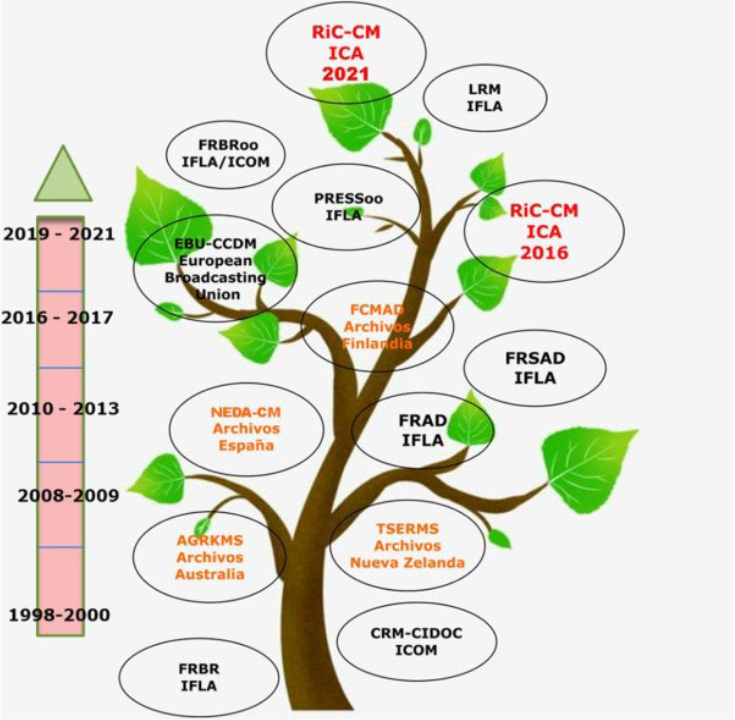
\includegraphics[scale = 0.4]{evolution_CM.png}
    \caption {L'évolution des modèles conceptuels/sémantiques. Issu de D. Llanes Padrón et M. Moro Cabero.}
    \label{fig:enter-label}
\end{figure}
\newline
\chapter{Le \textit{Record in Contexts standard}}
Le Record in Contexts (RiC) est un standard développé pour moderniser et améliorer la description archivistique, répondant à la nécessité de s'adapter aux défis posés par l'ère numérique\autocite{Duranti2001Impact, Taylor1987Transformation, MacNeil2007ArchivalTheory}. Il se présente en deux versions principales : RiC-CM (Conceptual Model) et RiC-O (Ontology). Ces deux versions, bien que complémentaires, répondent à des besoins et des défis spécifiques dans le domaine de l'archivistique et de la gestion des documents.

\subsection{RiC-CM (Record in Contexts - Conceptual Model)}

Le RiC-CM, introduit comme un modèle conceptuel, vise à fournir un cadre théorique pour la description archivistique. Il s'efforce de capturer et de représenter la complexité des documents d'archives et de leurs contextes de création et d'utilisation, soulignant la nécessité de moderniser la description archivistique pour mieux refléter ces complexités. Ce modèle met l'accent sur les relations entre les documents, les individus, les organisations et les fonctions, offrant ainsi une vision plus holistique et interconnectée des archives\autocite{ICA2016}. Le RiC-CM est conçu pour être suffisamment flexible pour s'adapter aux diverses pratiques et traditions archivistiques à travers le monde, tout en favorisant une plus grande cohérence et interopérabilité entre les systèmes de description archivistique.

\subsection{RiC-O (Record in Contexts - Ontology)}

Le RiC-O, quant à lui, est une ontologie formelle basée sur le modèle RiC-CM. Elle vise à traduire les concepts et les relations définis dans le RiC-CM en un format qui peut être directement utilisé et interprété par les systèmes informatiques, facilitant ainsi l'intégration des descriptions archivistiques dans le web sémantique\autocite{ICARiCOv02}. En adoptant les standards du web sémantique, RiC-O offre une approche plus dynamique et interconnectée de la gestion des archives, permettant une recherche et une récupération plus efficaces des informations.

\subsection{Défis soulevés et applications}

L'implémentation de RiC-CM et RiC-O présente plusieurs défis, notamment la nécessité d'aligner ces nouveaux standards avec les systèmes existants, souvent construits sur des modèles plus anciens et moins flexibles\autocite{Duranti2001Impact}. De plus, la formation et l'adaptation des professionnels aux nouvelles pratiques et technologies représentent un autre défi important.

La modernisation de la description archivistique est motivée par plusieurs facteurs clés. Premièrement, l'ère numérique a radicalement changé la manière dont les documents sont créés, conservés et utilisés, nécessitant une approche plus dynamique et intégrée pour leur gestion et leur préservation. Deuxièmement, les archives traditionnelles sont confrontées à l'immense défi de gérer des volumes croissants de données numériques, ce qui exige des méthodes plus sophistiquées pour la classification, le stockage et la récupération de ce type d'informations. Enfin, la nécessité d'améliorer l'accessibilité et la sérendipité des archives pour un public plus large et diversifié encourage la mise en place et l'adoption de standards comme les RiC-CM et RiC-O.

\subsubsection{Perspectives Futures}
Ces standards offrent également des opportunités pour des applications innovantes, telles que l'intégration de l'intelligence artificielle pour l'analyse et la classification automatique des archives\autocite{Spina2023AI, ColavizzaBlankeJeurgensetAl2021}.

\subsection{Quelques critiques}
Bien que le Record in Contexts (RiC) représente une avancée significative dans la description archivistique, plusieurs critiques et problèmes ont été soulevés par des professionnels du domaine.

Certains professionnels de l'archivistique soulignent le problème de financement et de possibilité de mise en oeuvre de moyen pour mettre en place ces nouveaux modèles. Cette complexité peut entraîner des difficultés dans la formation du personnel et dans l'adaptation des systèmes existants pour se conformer aux nouvelles normes. La flexibilité offerte par RiC-CM, bien qu'avantageuse pour s'adapter à divers contextes, pourrait également conduire à une absence de cohérence dans son application à travers différentes institutions.
Par ailleurs, bien que RiC vise à améliorer l'accessibilité des archives, la mise en œuvre de technologies avancées pourrait créer un fossé entre les institutions disposant de ressources suffisantes et celles qui en manquent\autocite{RokeTillman2022PragmaticPrinciples}..

.
\chapter{Conclusion}
En conclusion, notre exploration du développement et de l'application d'ontologies dans le contexte archivistique révèle une discipline en pleine mutation, façonnée par les avancées technologiques et les exigences croissantes de l'ère numérique et soulignant comment cette discipline, enracinée dans des pratiques anciennes, a évolué avec les sociétés qui la façonnent. 

Le concept du web sémantique a été examiné pour sa capacité à étendre les fonctionnalités du web actuel, en facilitant l'accès et l'interopérabilité des données. Cela a souligné l'importance de la standardisation des données et la pertinence des langages comme RDF et OWL dans la structuration et la connexion des informations.

L'analyse des ontologies a offert une perspective double : d'une part, une exploration de ses racines philosophiques, et d'autre part, son application pratique en informatique et en intelligence artificielle. Cette transition de la philosophie à l'informatique a révélé comment les concepts philosophiques ont influencé les développements technologiques, en particulier dans le domaine de l'IA symbolique.

Nous avons également observé le passage des modèles classificatoires traditionnels aux modèles conceptuels dans le domaine du patrimoine culturel, en mettant en évidence le rôle crucial des modèles conceptuels dans la gestion de l'information et l'interopérabilité des systèmes d'information culturelle.

Au coeur de cette mutation se trouve dans le contexte de l'archivistique le modèle RiC-CM et RiC-O. Bien que ces standards représentent une avancée significative, ils ne sont pas sans défis, notamment en termes d'alignement avec les systèmes existants, de financement, et de formation des professionnels.

Enfin, nous avons abordé les critiques soulevées à l'égard du RiC, mettant en exergue les préoccupations concernant sa complexité et les inégalités potentielles dans son application.

Ainsi, notre article conclut que bien que les standards tels que RiC représentent des pas en avant dans la modernisation de l'archivistique, ils exigent une réflexion continue, une adaptation et une prise en compte des défis pratiques et éthiques. Ces développements, bien que prometteurs, doivent être balancés avec une approche pragmatique pour assurer une application équitable et efficace dans le domaine toujours en évolution de l'archivistique et de la gestion des données.

\printbibliography
\end{document}
